Optical information is gathered by most animals through their eyes. 
The eye can be treated as a camera (Figure \ref{eye-schematics}): 
the cornea, iris, pupil and lens can be viewed as the mechanical 
lens found in commercial cameras. Light rays are bent and
focused on the ``\emph{film}'' or ``\emph{sensor}'',  
the \emph{retina} in the eye.
\begin{figure}[hbt]
    \centering
      \begin{subfigure}[b]{0.36\textwidth}
        \centering
        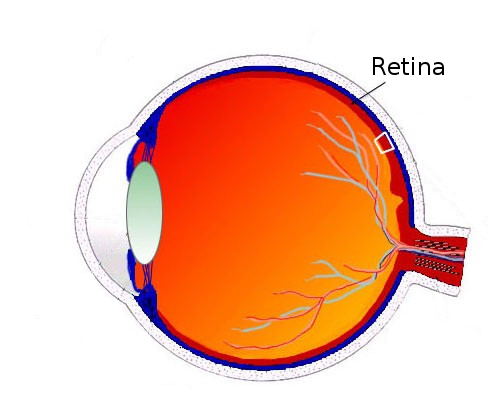
\includegraphics[width=\textwidth,valign=t]{Sagschem}
        \caption{Eye schematics}
        \label{eye-schematics}
      \end{subfigure}
      \begin{subfigure}[b]{0.32\textwidth}
          \centering
          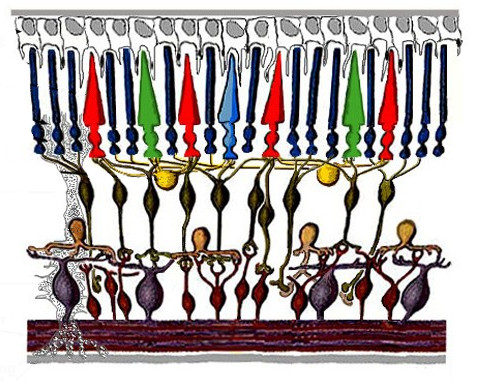
\includegraphics[width=\textwidth,valign=t]{schem}
          \caption{Retina}
          \label{retinal-layers}
      \end{subfigure}
      \begin{subfigure}[b]{0.3\textwidth}
          \centering
          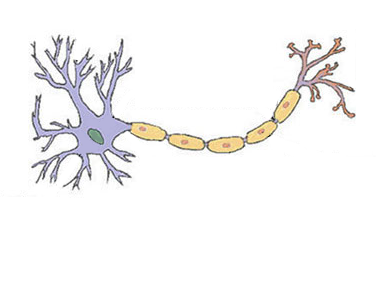
\includegraphics[width=\textwidth,valign=t]{Neuron-___-wikimedia-org}
          \caption{Neuron}
          \label{neuron}
      \end{subfigure}
            
    \caption{Anatomy of the (human) eye }
    \label{basic-eye-anatomy}
\end{figure}


Once the light enters the retina, it moves through several layers 
of neurons \cite{webvision} and hits the \emph{photoreceptors} 
(shown at the top of Fig. \ref{retinal-layers} \cite{wiki-images}). Light will 
elicit a chain reaction that has several steps, all occurring in 
the retina. On the central regions of the retinal layer there's a zone
called the \emph{Fovea}. The Fovea includes a small 
portion which is highly packed 
with \emph{cones} \cite{webvision-midget}, and has almost direct 
exposure to light, this region is known as the \emph{Foveal Pit}. 
This is the zone where images are acquired at the highest resolution.

The final step of the processing in the retina is carried out by 
\emph{ganglion cells} (bottom of Fig. \ref{retinal-layers}), 
this cells will emit spikes when certain 
conditions are met in the previous layers of the retina. The most
common type of cells are the \emph{Midget ganglion cells}. They 
are classified, depending on their input connectivity (dendritic
tree, left side of Fig. \ref{neuron}), as \emph{ON-centre} or 
\emph{OFF-centre} \cite{basab-thesis, webvision-midget}. 
What this means is that, an ON-centre cell will emit a spike
when the input in the ``centre'' region is stimulated but the 
surrounding area is not so much. The inverse case is true for 
OFF-centre type cells. The retina also contains another type
of ganglion cells whose dendritic trees span at much longer
distances, thus sampling wider portions of the image in the eye.
This last type of cells are called \emph{Parasol ganglion cells}
and come in both ON-centre and OFF-centre variants.





